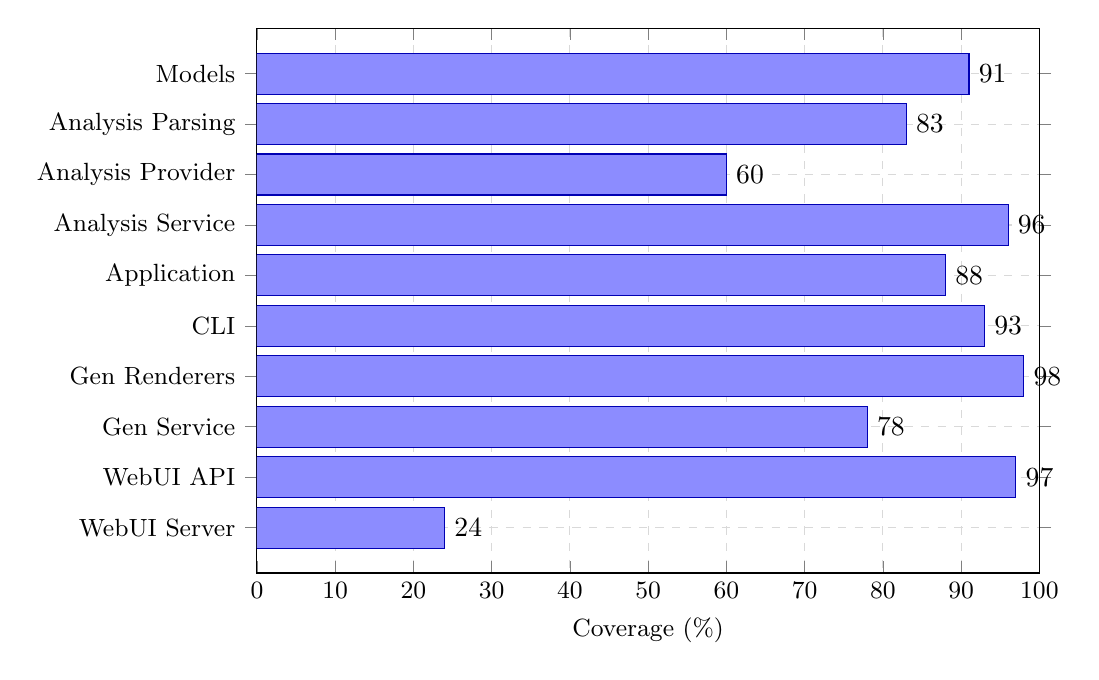
\begin{tikzpicture}
\begin{axis}[
    width=0.95\linewidth,
    height=8.5cm,
    xbar,
    xmin=0,
    xmax=100,
    xlabel={Coverage (\%)},
    symbolic y coords={{Models},{Analysis Parsing},{Analysis Provider},{Analysis Service},{Application},{CLI},{Gen Renderers},{Gen Service},{WebUI API},{WebUI Server}},
    ytick=data,
    y dir=reverse,
    bar width=0.52cm,
    nodes near coords,
    nodes near coords align={horizontal},
    grid=major,
    grid style={dashed,gray!30},
    tick label style={font=\small},
    label style={font=\small},
]
\addplot[fill=blue!45, draw=blue!70!black] coordinates {
        (91,{Models})
        (83,{Analysis Parsing})
        (60,{Analysis Provider})
        (96,{Analysis Service})
        (88,{Application})
        (93,{CLI})
        (98,{Gen Renderers})
        (78,{Gen Service})
        (97,{WebUI API})
        (24,{WebUI Server})
};
\end{axis}
\end{tikzpicture}
